\documentclass[11pt,a4paper]{../tutorial}
\usepackage[hidelinks]{hyperref}

\title{Tutorial 2 --- Adding FMUs}
\date{December 2017}
\author{Ken Pierce and Richard Payne}

\begin{document}

\section*{Overview}

This tutorial will show you how to:

\begin{enumerate}[noitemsep]
\item Edit a multi-model configuration
\item Add a new FMU to a multi-model configuration
\item Execute a co-simulation using the new multi-model configuration
\end{enumerate}

\section*{Requirements}

This tutorial requires the following tools from the INTO-CPS tool chain to be installed:

\begin{itemize}[noitemsep]
\item INTO-CPS Application
\item COE (Co-simulation Orchestration Engine) accessible to the Application
\end{itemize}

You may have been provided with tools and tutorials on a USB drive at your training session. Otherwise: 
\begin{itemize}[noitemsep]
\item Follow Tutorial 0 with the guidelines to install the INTO-CPS Application and COE.
\item Ask your instruction for the tutorial materials. These are available for students and members of the INTO-CPS Association\footnote{\url{https://into-cps.org/}}.
\end{itemize}



\section{Opening a Project}

\begin{instructions}
\item Launch the \emph{INTO-CPS Application}. On first loading, it will look like the screenshot below. If you have opened a project previously, that project will be opened automatically.

\begin{annotation}[width=0.85\linewidth]{figures/blankApp}
\end{annotation}

\item To open a project, select \emph{File \menusep Open Project}.

\begin{annotation}[width=0.85\linewidth,trim=0 260 0 0,clip]{figures/fileMenu}
    \usquare{4.6cm}{0.3cm}{0.1}{Open Project}{0.184,0.6}
\end{annotation}

\item Find \emph{Tutorials\pathsep{}tutorials\_2}, select it and press \emph{Select Folder}.

\begin{annotation}[width=0.85\linewidth]{figures/projectBrowser2}
    \usquare{2.2cm}{0.25cm}{0.8}{Browse...}{0.75,0.075}
\end{annotation}

\item Once the project is opened, you will see that project browser on the left of the INTO-CPS Application window is now populated. The entries in the project browser correspond to folders and files in the \emph{Tutorials\pathsep{}tutorials\_2} folder. These are:

    \begin{description}[noitemsep]
        \item[FMUs] Compiled FMUs (with file extension .fmu) that are used in co-simulation.
        \item[Models] Source models used to generate the FMUs. The icon of each entry shows which tool created the model. In this case Overture and 20-sim.
        \item[Multi-models] Used to configure co-simulations, including which FMUs are used and other co-simulation settings.
        \item[SysML] Architectural models that are used to create model and multi-model descriptions.
    \end{description}

    \begin{annotation}[height=0.64\linewidth,trim=0 0 250 0,clip]{figures/into_openedProject}
        \lpoint{0.81}{Compiled FMUs}{0.03,0.81}
        \lpoint{0.81}{}{0.03,0.77}
        \lpoint{0.487}{20-sim models}{0.03,0.487}
        \lpoint{0.487}{}{0.03,0.441}
        \lpoint{0.395}{VDM model}{0.03,0.395}
        \lpoint{0.301}{Multi-model configuration}{0.03,0.301}
        \lpoint{0.21}{SysML model}{0.03,0.21}
    \end{annotation}

\end{instructions}

This multi-model is a line-following robot, which contains a model of the body (including wheels and motors), a model of the sensors, and a controller which reads the sensors and controls the motors to make the robot follow the line.

\section{Editing a Multi-model}

In this tutorial, the controller FMU has not been added to the multi-model, and multi-model parameters are missing. We will add the FMU, set the parameters, then run a co-simulation.

\begin{instructions}
\item Double-click the \emph{mm-3DRobot} to open it.

    \begin{annotation}[width=0.53\linewidth,trim=0 0 250 200,clip]{figures/into_openedProject}
        \lsquare{2.4cm}{0.3cm}{0.5}{\hspace{2.6em}Open multi-model}{0.16,0.5}
    \end{annotation}

\newpage
\item Click on \emph{Configuration} to expand it.

    \begin{annotation}[width=0.8\linewidth]{figures/into_configure_mm1}
        \dsquare{8.2cm}{0.3cm}{0.62}{Configuration}{0.62,0.15}
    \end{annotation}

In the \emph{Overview} part an overview of the already configured connections is provided. This corresponds to the blue arrows in Figure~\ref{fig:initialconfig}.

\begin{figure}[!htb]
  \vspace{-0.2cm}
  \centering
  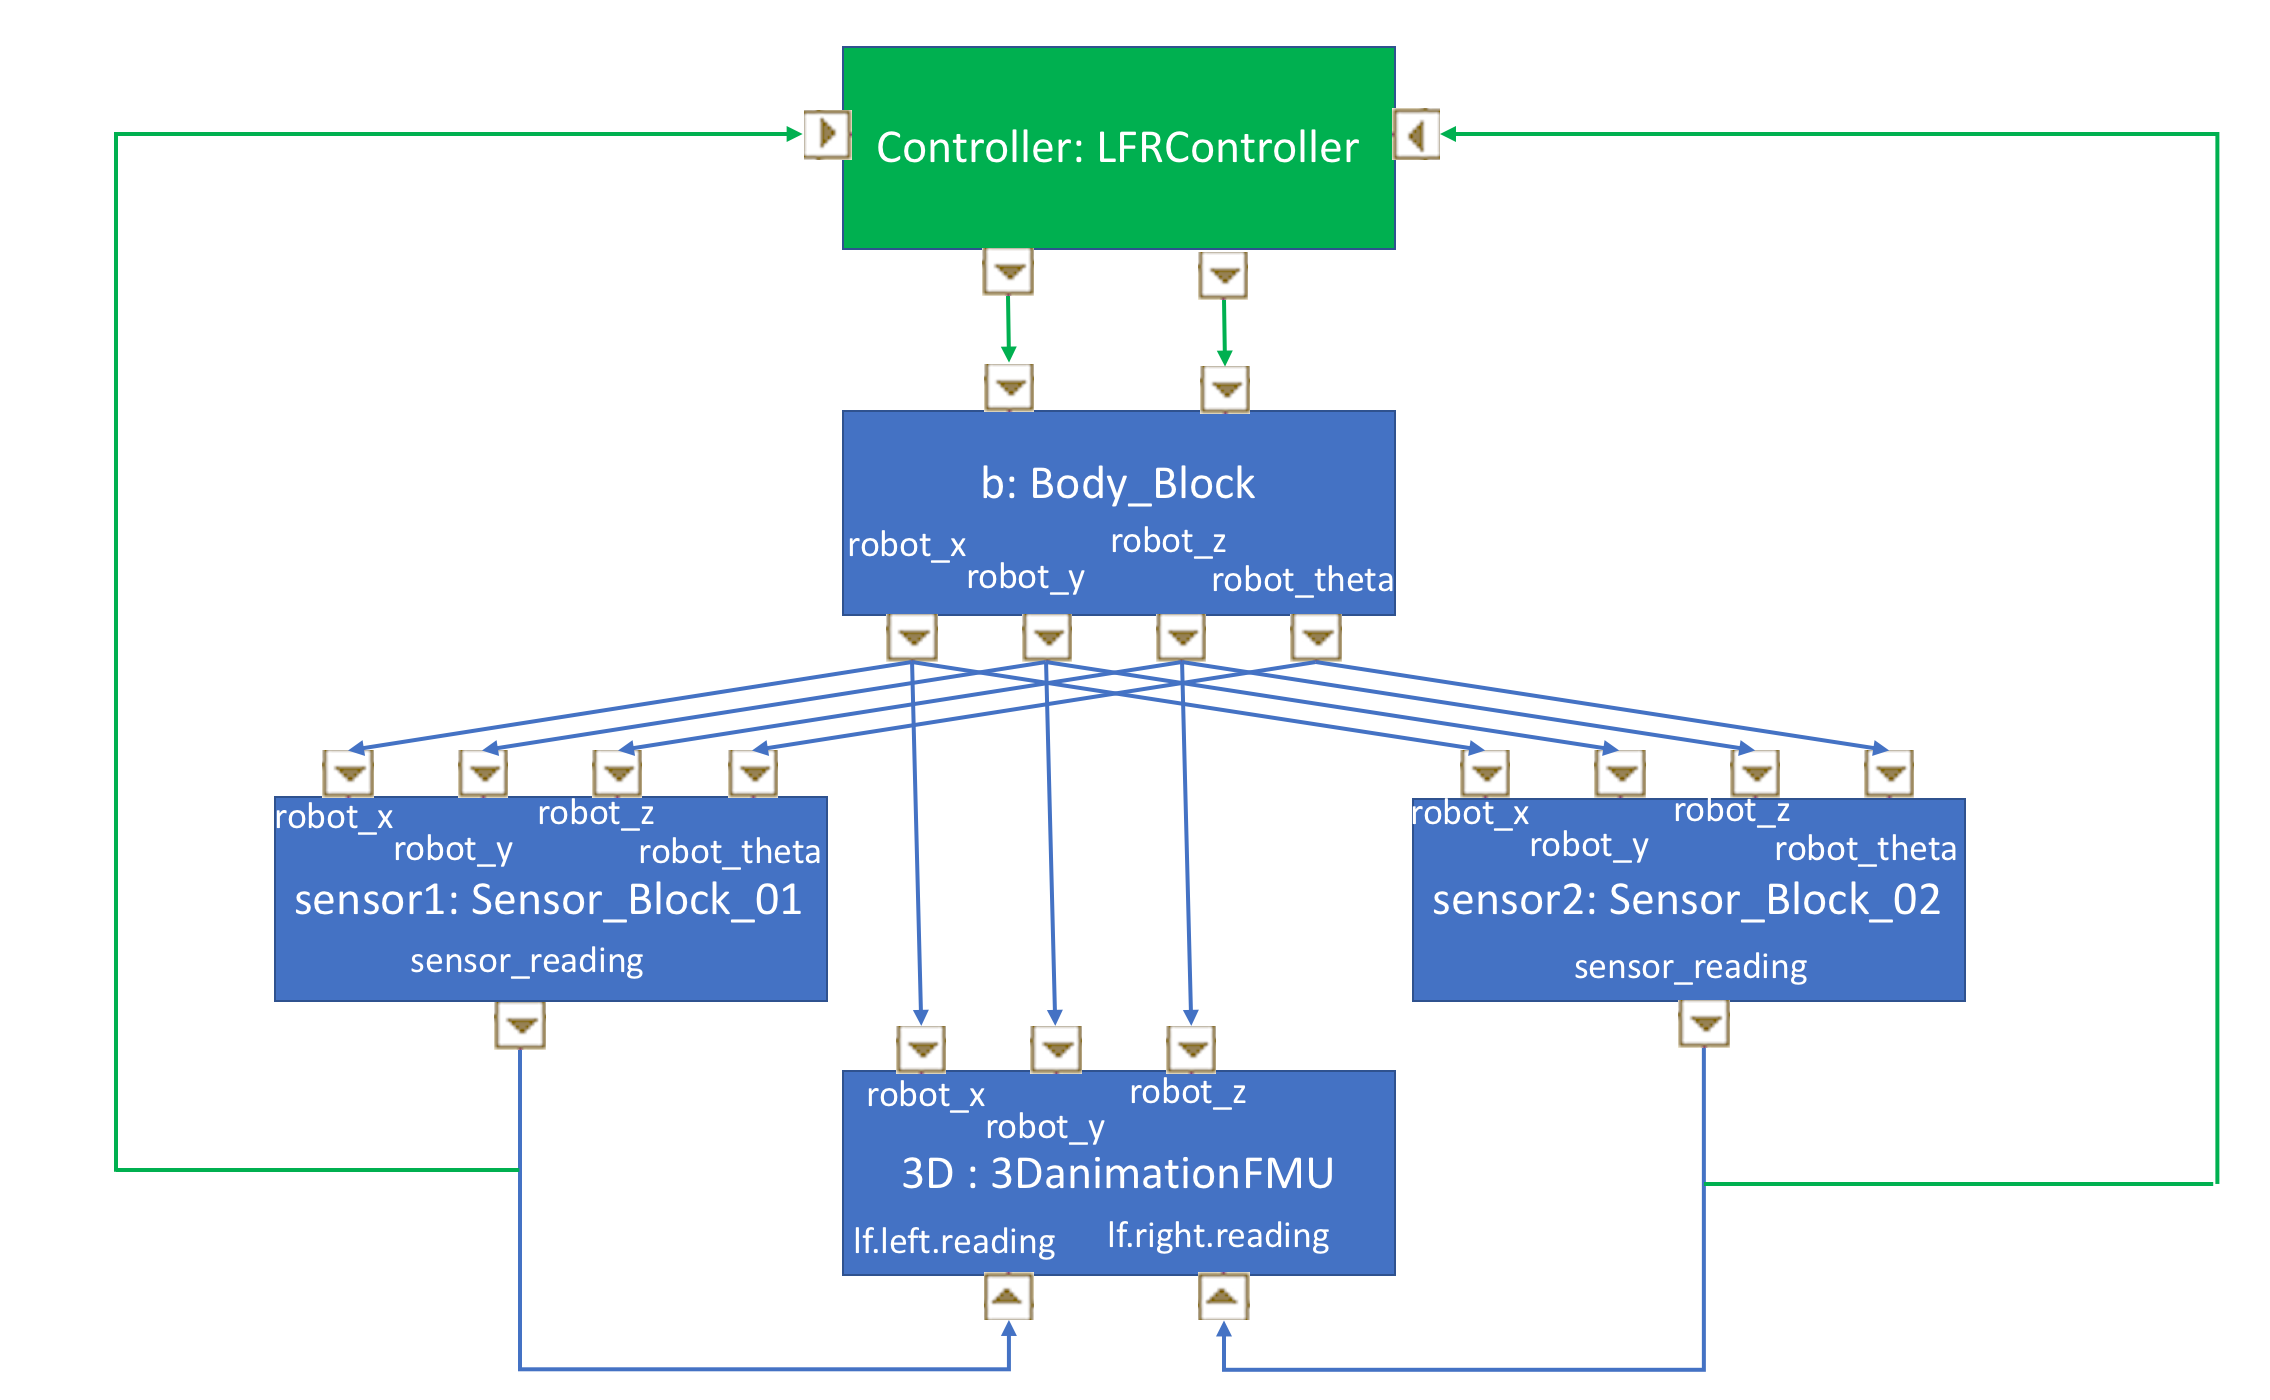
\includegraphics[width=0.9\textwidth,trim={6mm 5mm 6mm 5mm},clip]{figures/InitialConfigurations}
  \caption{Initial connections with blue, new ones to configure with green}
  \label{fig:initialconfig}
%  \vspace{-0.1cm}
\end{figure}
The green box and arrows in Figure~\ref{fig:initialconfig} are what you need to configure in the steps below.

\item Click \emph{Edit}.

    \begin{annotation}[width=0.8\linewidth,trim=0 0 0 250,clip]{figures/into_configure_mm2}
        \dsquare{1.1cm}{0.3cm}{0.4}{Edit}{0.33,0.87}
    \end{annotation}

\item Click the \emph{+} icon to add a new FMU entry.

    \begin{annotation}[width=0.8\linewidth,trim=0 120 0 250,clip]{figures/into_configure_mm3}
        \dcircle{0.25cm}{0.4}{Add FMU}{0.37,0.44}
    \end{annotation}

\item The new entry is named \emph{FMU}. Rename it to \emph{controller}.

    \begin{annotation}[width=0.8\linewidth,trim=0 0 0 250,clip]{figures/into_configure_mm4}
        \dsquare{3.2cm}{0.3cm}{0.4}{Rename to \emph{controller}}{0.415,0.55}
    \end{annotation}

\item We need to associate an FMU with this entry. To do this, click the \emph{File} button.

    \begin{annotation}[width=0.8\linewidth,trim=0 0 0 250,clip]{figures/into_configure_mm4}
        \dsquare{0.8cm}{0.3cm}{0.7}{File}{0.825,0.42}
    \end{annotation}


%\section{Creating a Multi-model}
%
%\begin{instructions}
%\item In the SysML entry of the project browser, expand the \emph{LineFollowRobot} and then \emph{config} folders. There should be a \emph{3DRobot} icon (as in the Figure below). Right click on \emph{3DRobot}, select \emph{Create Multi-Model}. You can just accept the default name in the prompt that appears.
%
%    \begin{annotation}[width=0.5\linewidth,trim=0 300 300 300,clip]{figures/into_create_mm}
%    \rpoint{0.7}{Expand to locate \emph{3DRobot}}{0.4,0.6}
%    \rsquare{3cm}{0.5cm}{0.5}{Create Multi-model}{0.47,0.5}
%    \end{annotation}
%
%\item A new multi-model configuration has been created and is shown in the multi-model entry of the project browser. Double-click on the new multi-model to open it.
%
%    \begin{annotation}[width=0.85\linewidth,trim=0 400 0 250,clip]{figures/into_new_mm}
%    \usquare{3.3cm}{0.5cm}{0.2}{Double-lick to open}{0.126,0.47}
%    \end{annotation}
%
%\newpage
%\item We need to associate FMUs with this multi-model and set its parameters. Expand the \emph{Configuration} section of the multi-model by clicking on the triangle.
%
%    \begin{annotation}[width=0.85\linewidth,trim=0 0 0 250,clip]{figures/INTOExpandConfig}
%        \dcircle{0.15cm}{0.8}{Expand \emph{Configuration}}{0.938,0.148}
%    \end{annotation}
%
%    \item Scroll down and click \emph{Edit}.
%
%    \begin{annotation}[width=0.85\linewidth,trim=0 0 0 250,clip]{figures/INTOEditConfig}
%        \dsquare{1.1cm}{0.12cm}{0.8}{\emph{Edit} configuration}{0.332,0.44}
%    \end{annotation}
%
%\item In the \emph{FMUs} section, next to the \emph{Controller} element \emph{c}, click the \emph{File} button.
%
%    \begin{annotation}[width=0.85\linewidth,trim=0 600 0 100,clip]{figures/into_add_controller_fmu}
%    \upoint{0.2}{Controller element \emph{c}}{0.3,0.64}
%    \usquare{1.1cm}{0.25cm}{0.7}{Click \emph{File}}{0.822,0.438}
%    \end{annotation}
%
%\newpage

\item A file browser window will open and show five FMUs (if the file browser does not show the FMUs, navigate to \emph{tutorials\_2\pathsep{}FMUs}). Select \emph{FMUController.fmu} and click \emph{Open}.

%\item The LFRController has been added. Repeat this for the remaining elements:
%
%    \begin{itemize}[noitemsep]
%        \item \emph{b} : \emph{Body\_Block.fmu}
%        \item \emph{3D} : \emph{3DanimationFMU.fmu}
%        \item \emph{sensor1} : \emph{Sensor\_Block\_01.fmu}
%        \item \emph{sensor2} : \emph{Sensor\_Block\_02.fmu}
%    \end{itemize}
%
%    \begin{annotation}[width=0.54\linewidth,trim=150 0 0 0,clip]{figures/INTOFMUsDone}
%    \rsquare{7.7cm}{10.8cm}{0.58}{All FMUs added}{0.484,0.47}
%    \end{annotation}

    \begin{annotation}[width=0.8\linewidth]{figures/FMUFindFile}
        \upoint{0.37}{1. Locate and select \emph{FMUController.fmu}}{0.3,0.52}
        \dsquare{1.5cm}{0.12cm}{0.63}{2. Click \emph{Open}}{0.788,0.0758}
    \end{annotation}

\newpage
\item The controller FMU is now associated.

    \begin{annotation}[width=0.8\linewidth]{figures/into_configure_mm5}
        %\dsquare{0.8cm}{0.3cm}{0.7}{File}{0.825,0.42}
    \end{annotation}

\item \textbf{MacOS X / Linux Only:} As in the first tutorial, the 3D visualisation FMU from this multi-model is only supported on Windows. Therefore delete it using the \emph{X} button.

    \begin{annotation}[width=0.8\linewidth,trim=0 0 0 0,clip]{figures/into_delete_3d}
        \dcircle{0.3cm}{0.2}{Delete FMU}{0.31,0.15}
    \end{annotation}

\newpage
\item Next we must add an instance of the controller. Under \emph{FMU Instances} click \emph{\{controller\}} then click the \emph{+} icon.

    \begin{annotation}[width=0.8\linewidth]{figures/into_configure_mm6}
        \usquare{7.8cm}{0.3cm}{0.2}{1. Click \{controller\}}{0.62,0.493}
        \rcircle{0.25cm}{0.4}{2. Add Instance}{0.39,0.415}
    \end{annotation}

\item Next the controller outputs must be connected to the body inputs (to control the motors). Scroll down to \emph{Connections}. Under \textbf{Output instance} click on \emph{\{controller\}.controllerInstance} and under \textbf{Output variable} select \emph{servoLeftVal}.

    \begin{annotation}[width=0.8\linewidth,trim=0 0 0 100,clip]{figures/into_configure_mm7}
        \usquare{7.8cm}{0.3cm}{0.62}{\{controller\}.controllerInstance}{0.62,0.47}
        \rsquare{7.8cm}{0.3cm}{0.3}{servoLeftVal}{0.62,0.3}
    \end{annotation}

\item Then under \textbf{Input instance} select \emph{\{b\}.b} and under \textbf{Input variable} check \emph{servo\_left\_input}.

    \begin{annotation}[width=0.8\linewidth,trim=0 70 0 0,clip]{figures/into_configure_mm8}
        \usquare{7.8cm}{0.3cm}{0.62}{\{b\}.b}{0.62,0.36}
        \rsquare{7.8cm}{0.3cm}{0.13}{servo\_left\_input}{0.62,0.13}
    \end{annotation}

\item Repeat the previous step to connect  \emph{\{controller\}.controllerInstance / servoRightVal} to \emph{\{b\}.b / servo\_right\_input}.

\item Then repeat to connect \emph{\{sensor1\}.sensor1 / lf\_1\_\_sensor\_reading} to \emph{\{controller\}.controllerInstance / lfLeftVal}.

    \begin{annotation}[width=0.8\linewidth,trim=0 165 0 0,clip]{figures/into_configure_mm9}
        \usquare{7.8cm}{0.3cm}{0.62}{\{sensor1\}.sensor1}{0.62,0.81}
        \rsquare{7.8cm}{0.3cm}{0.06}{lf\_1\_sensor\_reading}{0.62,0.06}
    \end{annotation}

    \begin{annotation}[width=0.8\linewidth,trim=0 0 0 126,clip]{figures/into_configure_mm10}
        \usquare{7.8cm}{0.3cm}{0.62}{\{controller\}.controllerInstance}{0.62,0.55}
        \rsquare{7.8cm}{0.3cm}{0.37}{lfLeftVal}{0.62,0.37}
    \end{annotation}

\item Finally, repeat to connect \emph{\{sensor2\}.sensor2 / lf\_1\_\_sensor\_reading} to \emph{\{controller\}.controllerInstance / lfRightVal}.

\item Next we must set the parameters of the controller, which determines how it responds to sensor input. Scroll down to \emph{Initial values of parameters} and select \emph{\{controller\}.controllerInstance}. Then click \emph{+ Add} for \emph{backwardRotate}.

    \begin{annotation}[width=0.8\linewidth]{figures/into_configure_mm11}
        \usquare{7.8cm}{0.3cm}{0.62}{\{controller\}.controllerInstance}{0.62,0.544}
        \rsquare{1cm}{0.3cm}{0.28}{Add}{0.915,0.28}
    \end{annotation}

\newpage
\item Set \emph{backwardRotate} to \emph{0.1}.

    \begin{annotation}[width=0.8\linewidth,trim=0 0 0 0,clip]{figures/into_configure_mm12}
        %\usquare{7.8cm}{0.3cm}{0.544}{\{controller\}.controllerInstance}{0.544,0.544}
        \rsquare{7.5cm}{0.3cm}{0.28}{0.1}{0.6,0.28}
    \end{annotation}

\item Use the drop-down box and \emph{+ Add} button to add:
    \begin{itemize}
      \item \emph{forwardRotate} with a value of \emph{0.5}.
      \item \emph{forwardSpeed} with a value of \emph{0.4}.
    \end{itemize}

    \begin{annotation}[width=0.8\linewidth,trim=0 0 0 0,clip]{figures/into_configure_mm13}
        \rsquare{1.4cm}{0.3cm}{0.375}{Add}{0.895,0.375}
    \end{annotation}

\newpage
\item \emph{Save} the \emph{Configuration}.

    \begin{annotation}[width=0.8\linewidth,trim=0 0 0 250,clip]{figures/into_configure_mm14}
        \dsquare{1.2cm}{0.3cm}{0.4}{Add}{0.335,0.34}
    \end{annotation}

%\item Next the sensor positions must be defined. Scroll down to the \emph{Initial values of parameters section}, and click \emph{\{sensor1\}.sensor1}. In the \emph{Parameters} section, enter the following values:
%
%    \begin{itemize}
%        \item \emph{lf\_position\_y} = 0.065
%        \item \emph{lf\_position\_x} = 0.01
%    \end{itemize}
%
%    \begin{annotation}[width=0.8\linewidth]{figures/INTOParams}
%        \dpoint{0.1}{\emph{lf\_position\_y}}{0.28,0.28}
%        \dpoint{0.5}{\emph{lf\_position\_x}}{0.42,0.15}
%    \end{annotation}

%  \begin{annotation}[width=0.7\linewidth,trim=0 0 0 400,clip]{figures/into_set_params}
%    \rpoint{0.7}{Parameters Section}{0.6,0.675}
%    \rpoint{0.5}{Select \emph{\{sensor1\}.sensor1}}{0.6,0.6}
%    \rsquare{7cm}{3cm}{0.2}{Set parameter values here}{0.6,0.275}
%%    \helpergrid
%    \end{annotation}
%
%\item Repeat the previous step for the second sensor -- \emph{\{sensor2\}.sensor2} with the following values:
%\begin{itemize}
%  \item \emph{lf\_position\_x} = -0.01
%  \item \emph{lf\_position\_y} = 0.065
%\end{itemize}

%\item \emph{Save} the \emph{Configuration}.
%
%    \begin{annotation}[width=0.85\linewidth,trim=0 0 0 250,clip]{figures/INTOSaveConfig}
%        \dsquare{1.25cm}{0.12cm}{0.5}{\emph{Save} configuration}{0.338,0.18}
%    \end{annotation}

\item The multi-model configuration is complete. Right-click on the multi-model configuration and select \emph{Create Co-simulation Configuration}. You can use the default name, \emph{co-sim}, or choose your own name.

    \begin{annotation}[width=0.85\linewidth,trim=0 0 0 0,clip]{figures/into_configure_cc1}
        \dsquare{3.85cm}{0.12cm}{0.5}{\emph{Create Co-Simulation Configuration}}{0.307,0.43}
    \end{annotation}

%    \begin{annotation}[width=0.85\linewidth,trim=0 120 0 130,clip]{figures/INTOCreateCoSim}
%        \dsquare{3.85cm}{0.12cm}{0.5}{\emph{Create Co-Simulation Configuration}}{0.293,0.52}
%    \end{annotation}

\newpage
\item Under \emph{Basic Configuration} set the the \emph{Step size} to 0.01. Don't forget to press \emph{Edit}.

    \begin{annotation}[width=0.85\linewidth,trim=0 70 0 0,clip]{figures/into_configure_cc2}
        \usquare{1.25cm}{0.12cm}{0.3}{\emph{Edit}}{0.335,0.66}
        \ucircle{0.15cm}{0.8}{Expand \emph{Configuration}}{0.943,0.747}
        \dpoint{0.7}{Set \emph{Step size}}{0.62,0.2}
    \end{annotation}

%    \begin{annotation}[width=0.85\linewidth,trim=0 0 0 0,clip]{figures/INTOSetSimTime}
%        \usquare{1.25cm}{0.12cm}{0.3}{\emph{Edit} then \emph{Save}}{0.338,0.81}
%        \ucircle{0.15cm}{0.8}{Expand \emph{Configuration}}{0.943,0.885}
%        \dpoint{0.7}{Set \emph{Step size}}{0.64,0.06}
%    \end{annotation}

\item Under \emph{Live Plotting} click \emph{Add Graph}.

    \begin{annotation}[width=0.85\linewidth,trim=0 0 0 30,clip]{figures/into_configure_cc3}
        \dsquare{2cm}{0.12cm}{0.3}{Add Graph}{0.37,0.22}
    \end{annotation}


\item Check \emph{lf\_1\_sensor\_reading} from \emph{\{sensor1\}.sensor1} and \emph{\{sensor2\}.sensor2} to see the sensor values appear in the \emph{Live\-stream Configuration}.

%    \begin{annotation}[width=0.85\linewidth,trim=0 230 0 250,clip]{figures/INTOPlotSensor}
%    \end{annotation}

    \begin{annotation}[width=0.85\linewidth,trim=0 200 0 0,clip]{figures/into_configure_cc4}
    \end{annotation}

\end{instructions}

\section{Running a Co-simulation}

\begin{instructions}

\item Launch the COE if necessary (see \emph{Tutorial 1 --- First Co-simulation} for a reminder if needed).

%    \begin{annotation}[width=0.85\linewidth,trim=0 270 0 120,clip]{figures/INTOLaunchCOE}
%        \usquare{1.25cm}{0.12cm}{0.8}{\emph{Launch} COE}{0.865,0.42}
%    \end{annotation}

    \begin{annotation}[width=0.85\linewidth,trim=0 110 0 200,clip]{figures/into_launch_new}
        \usquare{1.25cm}{0.12cm}{0.2}{\emph{Launch} COE}{0.355,0.35}
    \end{annotation}

\item When the COE is running (see \emph{Tutorial 1} if you need a reminder), click the \emph{Simulate} button. The graph should show blue and orange lines, and if these should move up and down, indicating that the robot is sweeping left and right, following the line.

    \begin{annotation}[width=0.85\linewidth,trim=0 30 0 35,clip]{figures/into_new_output}
        %\usquare{1.25cm}{0.12cm}{0.2}{\emph{Launch} COE}{0.355,0.35}
    \end{annotation}

\newpage
\item \textbf{Windows only:} During co-simulation, a Java window called \emph{Animation Frame} will appear like the one below. It shows a plot of variables from the co-simulation. You can click the \emph{3D} button to see the 3D visualisation of the robot.

    \begin{annotation}[width=0.5\linewidth,trim=0 0 0 0,clip]{figures/into_coe_3d_toggle}
        \rcircle{0.32cm}{0.8}{3D Button}{0.52,0.88}
    \end{annotation}

\item \textbf{Windows only:} A 3D model of the line following robot will appear. This view may be changed by clicking and dragging the mouse (note this is currently quite sensitive, so don’t make quick movements). When the simulation has finished, this window will close. If everything went well, the robot should follow the line.

    \begin{annotation}[width=0.5\linewidth,trim=0 300 0 0,clip]{figures/into_coe_3d_results}
    \end{annotation}

\end{instructions}

\section{Additional Exercises}

When this tutorial is complete, either move onto Tutorial 3, or try the following additional exercises:

\begin{enumerate}
  \item Experiment with different sensor positions. Repeat steps 13 and 14 to change the position of the left and right sensors relative the the robot body. How do the different values effect the simulation?
  \item Experiment with different robot speeds. Repeat steps 13 and 14 to change the different speed values for the \emph{Controller}. How do the different values effect the simulation?
\end{enumerate}

\end{document}
